\documentclass{report}

\usepackage{hyperref} % makes ToC clickable

% \usepackage{dnd}
\usepackage{eso-pic} % allows background picture patterning
\usepackage{graphicx} % \includegraphics
\usepackage[left=1in,top=1in,right=1in,nohead]{geometry}
% \usepackage{color} % Color DM only stuff
\usepackage{xcolor}
\usepackage{mdframed}
\usepackage{multicol}
\usepackage{tipa} % Ezh = \textyogh
\usepackage{etoolbox} % \ifdef / \ifundef for setting
\usepackage{fp} % For simple arithmetic / mod calculation
\usepackage{amsmath}
\usepackage{textcomp} % \textrightarrow
\hypersetup{
  colorlinks,
  linktoc=all,
  linkcolor=blue,
  urlcolor=black
}

\usepackage[colorinlistoftodos,prependcaption,textsize=tiny]{todonotes}   % adds \todo

\newif\ifdm
\dmtrue

\let\stdsection\section
\renewcommand{\section}{\clearpage\stdsection}

\newcommand{\dmonly}[1]{\ifdm{\color{blue}\hrulefill\par\textit{DM Only} #1\par\hrulefill}\else{}\fi}

\newcommand{\headeritem}[2]{\textbf{#1:} #2}

\newcommand{\race}[1]{\headeritem{Race}{#1}}
\newcommand{\class}[1]{\headeritem{Class}{#1}}
\newcommand{\voice}[1]{\headeritem{Voice}{#1}}
\newcommand{\player}[1]{\headeritem{Player}{#1}}

\newcommand{\STR}[1]{\renewcommand{\StrVal}{#1}}
\newcommand{\DEX}[1]{\renewcommand{\DexVal}{#1}}
\newcommand{\CON}[1]{\renewcommand{\ConVal}{#1}}
\newcommand{\INT}[1]{\renewcommand{\IntVal}{#1}}
\newcommand{\WIS}[1]{\renewcommand{\WisVal}{#1}}
\newcommand{\CHA}[1]{\renewcommand{\ChaVal}{#1}}

\newcommand{\statblock}[6]{\STR{#1}\DEX{#2}\CON{#3}\INT{#4}\WIS{#5}\CHA{#6}}

\newcommand{\modOf}[1]{%
\FPupn\unrounded{10.1 #1 - 2 swap /}%
\FPround\rounded\unrounded0%
\FPclip\result\rounded%
\FPifneg\result{%
\FPabs\absresult\result%
\FPround\rounded\absresult0%
\FPclip\newresult\rounded%
\texttt{-}\newresult%
}\else{%
\texttt{+}\result}\fi%
}

\newcommand{\reset}{
  \def\StrVal\undefined
  \def\DexVal\undefined
  \def\ConVal\undefined
  \def\IntVal\undefined
  \def\WisVal\undefined
  \def\ChaVal\undefined
}

\newcommand{\makeCharacterHeader}{%
  \begin{tabular}{cccccc}
    \stackrel{STR}{\StrVal(\modOf{\StrVal})} &
    \stackrel{DEX}{\DexVal(\modOf{\DexVal})} &
    \stackrel{CON}{\ConVal(\modOf{\ConVal})} &
    \stackrel{INT}{\IntVal(\modOf{\IntVal})} &
    \stackrel{WIS}{\WisVal(\modOf{\WisVal})} &
    \stackrel{CHA}{\ChaVal(\modOf{\ChaVal})}
  \end{tabular}
}

% \newenvironment{name}[args][default]{before}{after}
\newenvironment{aloud}{%
\begin{quote}%
\begin{sl}%
\begin{mdframed}[backgroundcolor=blue!10]
}{%
\end{mdframed}%
\end{sl}%
\end{quote}%
}
\newenvironment{character}[1]{
  \section{#1}
}{\reset}

\def\[#1\]{%
\begin{aloud}#1\end{align}%
}


\newcommand{\Enyhito}{Enyh\'{\i}t\H{o}}

\begin{document}

  \dmonly{{\LARGE
    This is the DM copy.
    If you're a player, this will have spoilers.
  }}

  \AddToShipoutPictureBG{
\includegraphics{parchment-paper-light-texture.png}}

  \tableofcontents

  \chapter{Foreword: Mechanics and Meta-information}

\section{Damage description}

Generally, I will call for you to describe your attacks hit.
However, in a fight it really only takes one or two solid hits with a weapon to kill someone.
To keep things at least half sensible with respect to how much damage a monster can soak, I'll use
  the following general guides when calling for the severity of blow your just dealt.

\begin{tabular}{|r|l|}
\hline
Remaining HP\dots & Described as \\
\hline
$0\%$    & Killing \\
$<25\%$  & Wounding \\
$<50\%$  & Connecting \\
$<75\%$  & Glancing \\
$<100\%$ & Absorbed \\
\hline
\end{tabular}

\newpage
\section{Speed Factor Initiative}

I'd like to use the Speed Factor Initiative rules with the Angry DM's modifier table.

For more, read:\newline\url{http://theangrygm.com/fine-i-wrote-about-speed-factor-initiative-in-dd-5e/}.

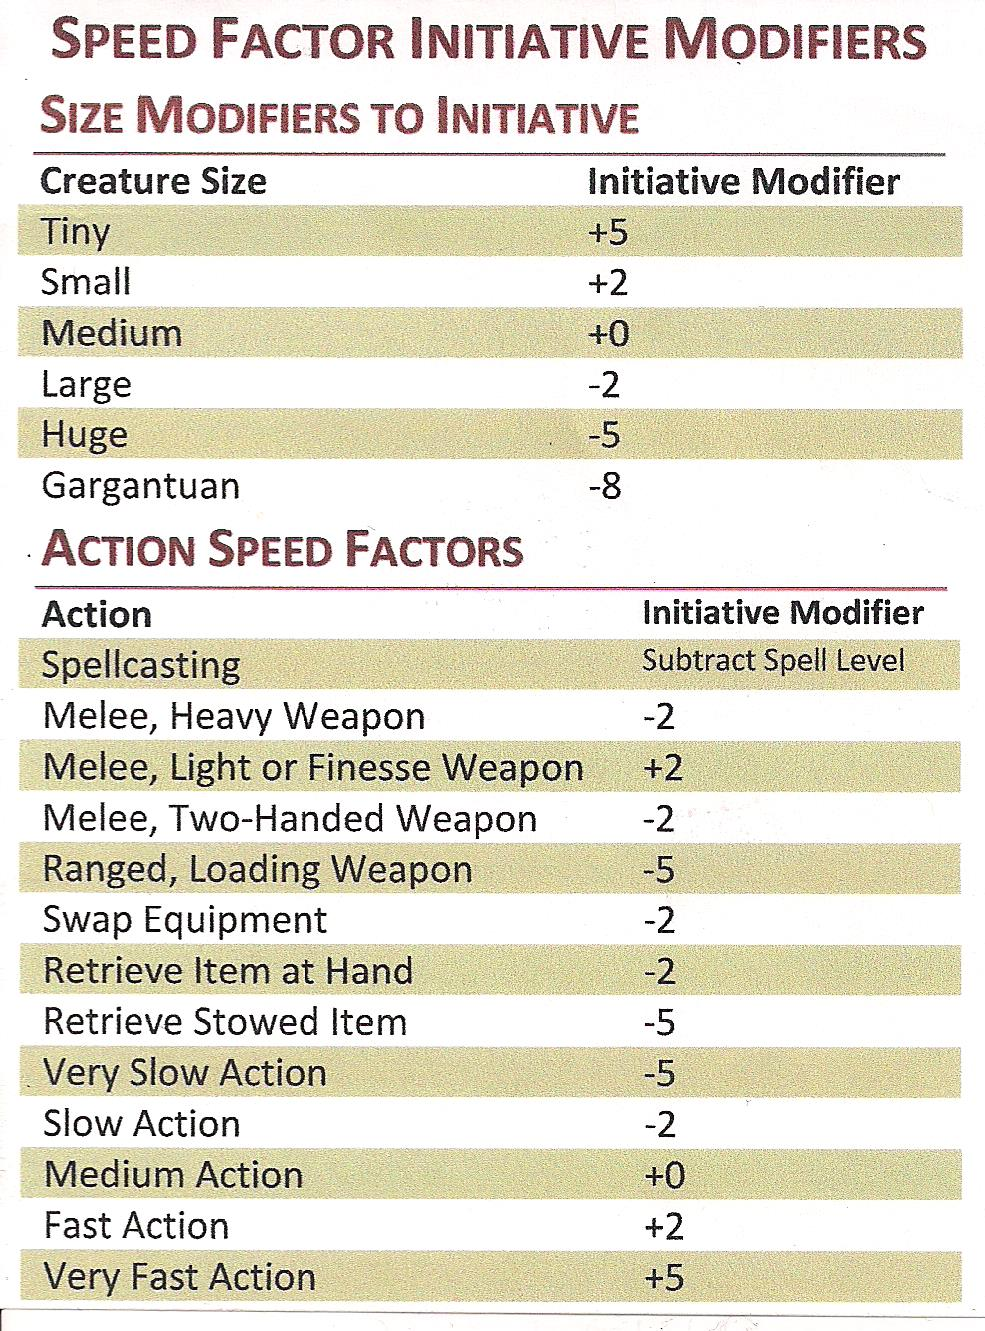
\includegraphics{img/speed-factor-initiative.jpeg}

\section{World map}
This is mostly as a note for me, but if it ever comes up on your next, a hex is 5 miles.
The PHB mentions that you can cover 18 / 24 / 30 miles a day at a slow / normal / fast pace,
  or 2 / 3 / 4 miles per hour.


\includegraphics[width=\linewidth,keepaspectratio=true]{img/maps/world-maps/Talaj.png}

\includegraphics[width=\linewidth,keepaspectratio=true]{img/maps/world-maps/Talaj2.png}


  \chapter{Setting}\label{ch:setting}

\chapter{Geography}\label{ch:geography}


\includegraphics[width=\textwidth]{img/maps/world-maps/Talaj.png}

\section{The Thornic Empire}
\headeritem{Structure}{Feudal Monarchy}

The yuan-ti established an empire but were driven out, slaughtered wholesale.
Some few escaped east, into the Tribal Wastes.

\subsection{Culture}
\subsubsection{Race Relations}
The Empire was founded in driving out the violent beast races.
While non- and half-humans are recognized all the rights of citizens, an attitude of human
 superiority pervades.

Elves are viewed as exotic novelties, despite many having been born and raised within Empire cities.
Half-orcs struggle to find work beyond menial labor.
Dragonborn, Aasimar and Tiefling tend to wear robes to keep their face and features hidden.

In cities, non-humans will have their own neighborhoods.
These aren't the slums common to third-class citizens, but intermixing is rare.

\subsection{Military}
Each baron must raise and maintain their own armed forces.
Each baron's force is divided into divisions.
A number of divisions are given to an impartial command, answerable only to the high Lord Admiral
 of The Empire and his Lord Marshals, in proportion to the size and population of the barony.
However, to discourage predictably disingenuous behavior in the peerage, the choice of which
 divisions serve The Empire and which are kept under the direction of the baron is made
 annually by the Lord Marshals.

\subsubsection{Armed Ranks}
Footman \textrightarrow
Knight \textrightarrow
Sergent \textrightarrow \ldots

\ldots \textrightarrow
In semi-limbo and generally self-supervised:
Warrant Officer, a title by a magistrate, decree, or other (generally political)
  appointment rather than rising through the ranks.
Typically has strings attached.

\ldots \textrightarrow
Lieutenant \textrightarrow
Captain

\ldots \textrightarrow These titles usually come with land, rights to council, etc:
Baron \textrightarrow
Lord Marshal \textrightarrow
High Lord Admiral

\subsection{Auxiliary Ranks}
Ensign \textrightarrow
Corporal \textrightarrow
Sub-captain

The sub-captain answers to a military captain but otherwise generally has free reign of operation.

\subsection{Arcane Ranks}
Apprentice \textrightarrow
Adept \textrightarrow
Erudite \textrightarrow
Master \textrightarrow
Grand Master

The Arcanum is never explicitly granted lands nor political council and is intended to be a
  neutral party.
There is a balancing act surrounding a Arcanum's obligation to military service with its holdings
  which are technically rented at the pleasure of the Emperess.

\section{The Northern Wylde}
\headeritem{Structure}{Desolation}

The farther north one travels, the more dense the forest becomes.
A small village, Dileah, is nestled in these woods, built up as a logging camp expanded outward.
This village and the roads from it mark the edge of The Empire's will and interest in the norther
  reaches.

A day's walk north of Dileah, scraps of white cloth dangle from tree limbs, another tied every
  dozen strides.
This ragged line traces roughly the line that which a cartographer would draw on a map.
Locals call this "the edge."
This marks the edge of The Empire's promise of protection.

Continue several hours farther, through thick bramble and undergrowth, and you would find
  bright red ribbons tied in a similar fashion.
These drift and snap in an unfelt wind, despite the heavy stillness of the woods.
They mark the edge of safety.

According to the folklore in Dileah and the surrounding villages, the "rag line" marks the territory
  of The Ragged Witch.
Most who cross the rag line are never seen again.
The few that return are found beaten, bloodied, gagged, and bound beneath one of the
  white scraps marking the edge.
These few will tell of a dark-skinned, gaunt figure clad in layer upon layer of tattered robes and
  cloaks.
Her voice strikes like iron, rebuking their trespass, shortly before darkness descends.

\section{The Southern Sea}
\headeritem{Structure}{Lawless}

Pirates and heavily-armed merchants.

\section{The Tribal Wastes}
\headeritem{Structure}{Fractured Clans}

Over the centuries, the beast tribes discovered in The Empire have been,
 if not slaughtered outright, driven east.
A partial misnomer, the Wastes are not a barren desert, but a lush grassland.
However, pockets of Gnolls, Goblins, Trolls, Orcs, Kobolds, Bullywugs, Lizardmen, and
 remnants of the once powerful Yuan-ti make travel into the Wastes lethal for almost
 all who enter it.

Aarakocra and Kenku tribes are also found in the Wastes.
These are often the only safe haven from an onslaught of violence that would befall those
 that must travel the Wastes.

\subsection{Boundary}
The Merlicut Gorge is maybe 1,500 feet across.
(Mississippi in the Quad Cities, give or take.)
Maybe short bridge to Arsenal Island with a redoubt, with the major bridge from there.



\subsection{Good monsters}

Axe Beak (CR: 1/4, Monster Manual p.317)

Blink Dog (CR: 1/4, Monster Manual p.318)

Blood Hawk (CR: 1/8, Monster Manual p.319)

Brown Bear (CR: 1, Monster Manual p.319)

Cockatrice (CR: 1/2, Monster Manual p.42)

Dire Wolf (CR: 1, Monster Manual p.321)

Elk (CR: 1/4, Monster Manual p.322)

Gnoll (CR: 1/2, Monster Manual p.163)

Goblin (CR: 1/4, Monster Manual p.166)

Harpy (CR: 1, Monster Manual p.181)

Hyena (CR: 0, Monster Manual p.331)

Orc (CR: 1/2, Monster Manual p.246)

Wolf (CR: 1/4, Monster Manual p.341)

Worg (CR: 1/2, Monster Manual p.341)

Yuan-ti Pureblood (CR: 1, Monster Manual p.310)



\section{The Western Horde}
\headeritem{Structure}{Hierarchical Magocracy}

Ruled by: The High Dragon, Ayanum.

Emissary: The Dragon's Breath, Mesheshi.

Dragonborn ruling class, humans are a short-lived pestilence.

Kasdiel



\chapter{Locations}\label{ch:locations}

\section{Celadir's Bastion}\label{sec:celadir'sBastion}
Bloo


Deadwood, Stalker, old town watchpoint turned gold rush.
most of what Ankh Morpork is built out of Ankh Morpork


Celadonian supports the old guard.
Influx of population provides a problem.


\section{The Norther Woods}\label{sec:theNortherWoods}
Blah



\chapter{Lore}\label{ch:lore}

\section{Stomah Thorne and the Four Defiant -- The Origin of the Empire}

\textit{This is a story told throughout the Empire, by bards in barrooms, by youths around
  campfires, and by parents (albeit less explicit) to their restless children.
While all of them -- bards, youths, and parents -- are notorious liars, the story of Stomah's
  march across the modern-day Empire is generally accepted as truth, within the bounds of
  exaggeration accepted as good story-telling.
While not going so far as to have their own temples, Stomah and The Four Defiant themselves are now
  revered almost as gods for their foundational importance to the Empire.}

\medskip

In the days before the Empire, we warred with the beastmen constantly.
Herders worried less about wolves taking sheep than they did about gnolls taking their lives.
Despair hung over the land like a heavy fog.
These dark, harsh times made dark, harsh people.
People like Stomah.

Stomah rose from the glowing embers of her ruined village with nothing but a sword and a promise:
  the beastmen would pay to their last.
The human traveled from town to town, taking the long and dangerous paths.
In her wake, the beast-tribes burned.
Gnolls lay be the roadside, gnarled and twisted.
Kobold caves filled with their fallen, each one cracked and broken.
Lizardmen lay lacerated.
Bullywug bodies bloated.

In time, Stomah's name would demand fear and reverence in equal parts.
In every city she would visit, every town, every village, every hamlet,
  men and women would join her.
They would make their own promises and take up their own weapons, for all had lost something
  to the beastmen.
Stomah would lead them, always along the long and dangerous paths, calling due every bloody debt.

Yet in those early days, before her host became her army, before her ruined home became the seat of
  an Empire and she our First Empress, before any of that, she was joined by a band
  -- the Four Defiant.
The Defiant had themselves crushed many beastmen under their collective heel,
  not for revenge but for profit.
The band of adventurers kept the area safe and themselves fed.
They were known as talented mercenaries, but altruists, they were not.

No one knows what Stomah said to bring them to her cause driving out the beastmen.
Certainly, she had no coin by which to hire them.
Perhaps she pleaded, her impassioned call fanning a hope the Defiant had themselves
  thought long smothered.
Perhaps they recognized in Stomah the last element.
With her, they would form an alloy no enemy could break.

Whatever the reason, the five left that western town of Breygrove on a long trek eastwards, toward
destiny.

\hrulefill

Stomah stands alone, her longsword held in both hands.
Three gnolls stand before her, yipping at her uncertainly.
Behind her, the bodies of other hyena mark where she has been.
Gnoll blood stains her hair and drips slowly into her eye.
The hyenamen sense the opportunity, attacking together, but even partially blinded, they are no
  match for Stomah.
She has led this dance so many times, it comes as easily as breathing.

Some distance away, Poise stands motionless in the center of a circle of the beastmen.
Her pale hair floats wild in the wind.
She holds no weapon.
She shouts no threat nor plea.
Her downcast eyes and small frame belie her threat.
She is the patient, ceaseless roll of the sea.
She is the undertow that drags the unwitting beyond the safety of shore to drown them there.

###

The Raven's laugh croaks sharply through the battlefield.
The Elf is old even among Elves.
Her skin like charcoal and ash is dusted with actual ash and smeared with sweat.
A gnoll charges at her, spear leveled.
Her tattered robes cover tattooed whorls, which whirl and roil when she work her spells.
In a flash of flame, the gnoll is gone, more ash filling the air.
The Raven's harsh laugh sounds again.

From atop a hastily-deployed palisade, a half-Orc balances precariously to watch his allies.
Soot and grease stain the Wrecker's leather gloves, leather apron, and rough leathery face.
The Wrecker could break a siege by himself, given enough time, iron, and wire.


His heavy work hammer and strong arm were deadly in a melee, but deadlier still in his workshop.









Celadir's understanding of combat let the Defiant predict every attack,
but it was often the Raven's magic that let them survive it.


Of the Four Defiant, only Celadir's name lives on.
The half-Elf would later be named Regent, though he wouldn't know it at the time
  and would come to renounce it in the end.
Stomah would hold Celadir foremost among her councilors,
  count him first of her few friends,
  and, some rumored, invite him alone to into the circle of her arms.
Throughout history both before and since, none can call themselves equal
  to Celadir's tactical genius.
It is said that for every life Stomah ended, Celadir's wisdom in battle saved dozens.

\hrulefill

And so the group traveled the roads that today mark the outskirts of our Empire.
Their name, fame, and fortune grew, and with that so too did their number.

Stomah and her warriors pressed onward.
Before their blades, the beastmen fell.
Before their wrath, the beastmen fled.

Stomah, the Defiant, and their host drove the beastmen east,
  toward the great and wild Rahlu River.
On they pressed them, to the ancient, wide bridge called the Bastion.

That night, they paused in their attack, Stomah and her forces on the western side of the Bastion,
  the dwindling number of beastmen on the east.



####
The host driven east.
Stomah pursued.
Celadir voiced concern about exposing themselves.
Stomah orders her four most trusted warriors, advisors, friends to stay.
The rest of the host pushes north.

The Yuan-ti, the serpent-men, are as devious as they are vile.
Stomah is assassinated.
The Yuan-ti descend upon the western banks of the river.
They are not prepared.

The Raven, The Wrecker, The Regent, The Wrath, score a line in the earth.
Those abominations that dared to cross it were mete a brutal reward.

The Yuan-ti horde flowed for ages, but the fervent fury of the four was unending.



  \chapter{Player Characters, aka The Group}

\section{Preface: Jo'am meets a stranger}\label{sec:joamMeetsAStranger}

\begin{multicols}{2}
  \subsection{A visit to Gran's}
  \begin{aloud}
  It's late morning on a pleasant mid-spring day.
  It rained last night, so you think today might be a good day for foraging.
  At some point, you wander towards Gran's.

  As you walk down her road, you pass a merchant in a cart coming from her house.
  It's strange, because hardly anyone is willing to come past the edge, this close to the rag line.
  A young human male is driving the cart.
  He's wearing a bright blue askot, a wide floppy hat, and otherwise simple travel fare.

  What happened: Jo'am pet the horse for a while, said ``Hello BlueMan.''
  Eventually got nudged out of the way.
  \end{aloud}

If Jo'am stops him, the merchant-boy Jerome will chat.
He crossed the rag line last night fleeing cultists.
The askot is gran's threat against him if he violates his $geas$.
If commented upon, he's lie, probably poorly, but not discussing it is part of the $geas$.
He is more than happy to sell Jo'am any simple fare he might ask for.


Continuing to Gran's:

  \begin{aloud}
  As you approach Gran's cottage, everything feels right.
  The bees are buzzing around their boxes, the goat is in his pen, goating.
  As you approach, you notice the front door is slightly ajar.

  What happened: Jo' let himself in, hollered a hello, but otherwise sat down to watch gran's game.
  \end{aloud}

Calling out gets no response.
Depending on Jo'am's reaction, he might interrupt the next bit.

  \begin{aloud}
  Gran is at her table in the middle of the room, muttering to herself and playing her
    funny card game.
  She looks up as you enter, nods at you and offers a flickering smile, but doesn't interrupt
    her game.
  This isn't the first time you've walked in while she's busy like this, and you know it won't
    take long for her to finish.

  What happened: Succeeded on most of the first spread, some of the second,
    just dungeon and demon of the third.  Maybe also Yuan'ti dreadlord.
  \end{aloud}

If he stays to watch, show him the cards.
Each stack should have a DC 12, +1 per card, for him to see a flicker of the future.

Afterwards, Gran chews her lip a bit.
Seeming distracted, she still greets Jo'am  properly, offers him what's left of breakfast or tea.
If asked about Jerome, she'll say he was just a passing merchant.
If pressed, she'll joke about how he must've sensed her charm even from the main road.

After a moment, she'll look over at her windowsill tangle and frown.
One of the threads has come loose and is flapping in the wind.
DC 12 WIS + INT to realize that there isn't any wind, which Jo'am has ``always thought funny''
that the tangle would do that.

Seconds later, another strand comes loose.
Gran curses.
The cards have been left out.
She glances between them, the tangle, and Jo'am.

``Could you do your gran a favor?
While you're out today, go check on your friend Smit.
If he's got any venison cured, I'd take as much as he's willing to sell.
Tell him it's my money so he doesn't cheat himself thinking he's doing you a favor.''

\begin{aloud}
What happened: Joam cleans up after himself, gathers his things carefully, takes the tangle
  because he's going to fix it.
\end{aloud}

\subsection{Wandering the Woods}

Try to gauge how distracted and noisy Jo'am is.
Perception to determine how far away his token is.
Ask if he's traveling along, in, or just kind of close to the stream.

Some distance away, he hears the sounds of struggle.
One man is standing in the stream, shouting at the other man.
``You agreed though, we both did.
  Are you a liar?
  We just have to do what it says.
  We have to.''
The other man is holding someone's head in the stream.
He is shounting, too.
``You have to take it, you have to, you have to, I want it out, he says he'll leave.
I changed my mind, I don't want it, get it out get-it-out getitout gititoutgititoutgititout!''

When they notice Jo'am, they are distracted and the man being held under surges free.
It is bound at the wrists.
It is Smit.

What do you do?

\begin{aloud}
  What happened: The drugs are starting to hit.
  Dig into a big rock, find some yummy moss.
  Hear splashing and shouting down the way.

  Smit and Crazy Man A tussle on the ground a bit.
  A swings and misses, driving his knife into the soft ground.

  Jo and Crazy Man B swing it out.
  Jo shouts about helping get rid of the bad spirits.
  B thinks he's going to help until a heavy, two-handed swing almost bowl him down.
  Alarmed, he stabs at Jo, glancing a blow off his walking staff but failing to bite into the meat of him.
  Jo responds more carefully this time, with a full-forced blow sideways across B's jaw.
  B holds his bleeding face, Jo kicks him into the stream.

  Meanwhile, Smit headbuts A's nose, spraying blood but otherwise not disabling A.
  Jo runs across to help.
  A, seeing this and his pummeled ally, scambles to his feet and starts to flee.
  Jo swings his staff and sends A stumbling to the ground.

  B has gotten to his feet.
  Jo asks ``Bad spirits gone?''
  B replies ``No, we agreed, he'll never leave, that's what we promised, we're not liars.''
  Jo goes to get rid of the bad spirits.

  Smit, seeing the man who held him in the stream mewling on the ground, delivers several kicks
    to A's head.
  Jo brings his staff down once more.
  With a sickening crack, B's face caves inward.
  Blood splatters.

  The drugs hit.
  Jo can feel every drop of blood spray across his face.
  Drop.  drop.  drop.
  One droplet lands in his eye, and the world turns red...
\end{aloud}

  \subsection{A guest}
As the last cultist dies, blood spatters into your face and mouth.
Time dilates.
Something is speaking to you inside your head.
It's different from how the spirits usually talk to you.
They usually use your own voice and words.
This one uses ideas to speak, but it's stumbling and jumbled.
With each phrase, you imagine something like the mess the bottom of a tankard leaves --
  a splattered circle -- and you know somehow that the different splatters are the phrases, too.


\begin{verbatim}
Self :: Joy ; Greeting > Start + Host
Self :: Optimism ~ Friendship < Host
Confidence . Secret && Incumbent + Host
< Dissatisfaction + Disappointment ~ Fragility
Observation && Host :: Fortitude < Compliment
Question && Host :: Willingness ~ Tenancy < Self
\end{verbatim}

After you accept, time seems to lurch back into place.
Smit is sitting, heaving breaths.

  \begin{aloud}
  What happened:  Pretty readily accepted the ``Blood Spirit'' into the back of his head.
  \end{aloud}

  \subsection{Aftermath}
Smit is shaken.
``They were going to kill me.''
Hopefully, Jo'am will help get him steady.

``See me home, would you?''
Recover a deer that Smit had shot.
He holds his knife and looks at the deer, unsteady.
``I don't suppose you can dress a deer?''
Maybe throw up in the stream.

Carry it the rest of the way down the stream to Smit's hut.
Or maybe they abandoned it.
Smit changes clothes.
Maybe they bum around a bit.
Smit goes stir crazy.
``Shomah's fucking fury, man.
  I'm going to the bar.
  You in?''

Play that scene by ear.

At some point, you go home.
Or not.
Maybe you're just wandering the woods now.
Let's find out.
But you cross the rag line, maybe on the shortcut you always take home, maybe on accident.

  \begin{aloud}
    What happened:
    Wander to smits shacks and cabin.
    Big man Jo has man-handled a deer carcass back to the shacks, where Smit hastily dressed it.

    They look the mess.
    gotta go to the bar.
    Jo puts on some of Smit's several-sizes-small clothes.

    On the way to town, Jo remembers to ask for cured venison.

    They get drunk.
    ``I met a blue man!''

    Stumble back to the cabin.
    Forget about the venison.

    Wander back half an hour later.
    Wake the loudly snoring Smit.
    Get some venison.
    Return to Gran's, after a full day.
  \end{aloud}

  \subsection{A Ragged Witch Appears}\label{subsec:scene:ARaggedWitchAppears}

  \begin{aloud}
  You look at the red ribbons hanging from the trees that mark the rag line.
  As you cross, they crack like they're in a gale wind.

  Her gravely voice seems to come from everywhere at once.
  ``You must know that to trespass means death.''
  You see her, the Ragged Witch, not far from you.
  Her tattered robes whip around her.
  ``My laws are absolute.''
  She lifts a hand at you, approaching closer.
  ``You have brought this on your own --
    Jo'am?!''

  Instantly, the winds die down.
  The tattered robe melts into gran's cloak.
  She runs up to you but stops short.
  ``Jo'am?''
  She looks you in the eye.
  ``What have you done to my Jo'am?''
  \end{aloud}

  \begin{aloud}
    What happened:
    ``Bad spirits out tonight gran.''
    Remembers to give venison and the ``fixed'' tangle.
  \end{aloud}


  Converse.

Gran is sad, but Jo'am has to leave.

``Will you come with me?''

Teleport.
You're on a road somewhere.
A cart is trundling down the path.
Gran gives Jo'am a bright red strip of cloth,
``As long as you keep this, I'll be watching over you.''

\subsection{On the road}\label{subsec:scene:OnTheRoad}
  Your driver has a lightning blue askot and a floppy hat.
  You head east.
\end{multicols}

\section{Traveling South and East}

Stop in a ``major city'' on the outskirts of [You still need the capital's name].
Maybe talk about the troublesome type that have been passing through lately.
This will have been 10 months after Goldie left the western front.
Nat sings Sera Never Was as you travel.
Maybe a Misty Step \emph{bampf}, and then Goldie introduces herself from atop the cart
  ``I love this song.''




Jo's hometown name: Shortspur

Saying: "Streams know where they flow."


%\section{Another day, another drink}
\begin{multicols}{2}
  \begin{aloud}
    It's early morning, mid-spring, and you're sitting at a table at the Last Shot.
    It's the end of your week back ``on shore.''
    The final preparations are being made, and you'll cross back into the wilds before lunch.

    Whitney, is recounting a story he'd heard this week,
      the \emph{real} story of how the some great wizard Merlin formed the Gash during the
      Bleak War hundreds of years ago.
    He looks like a merchant;
     everything about him is round.
    He has long curled hair, healthy bronze skin, and a gigantic braided beard.

    Your leader, Gluri Frosthand, is seated at the bar.
    Gluri has been in this town for as long as it's been worth being here.
    The dwarf is shaved bald, and his brown skin is perpetually sunburned a hint of red.
    He's got the ugliest goatee you've ever seen, and he love it.
    His right hand is missing the last two fingers.

    He's chatting up the bartender, Skril, and making final supply requests.
    She's one of those human contradictions.
    A glance at her, and you'd think she's the meanest bitch you'd ever met.
    Dark hair is shaved to stubble, her arms are crisscrossed with combat scars.
    She brooks no nonsense in her bar, and the way the town has been going, it's threatened to see
      plenty of nonsense these days.
    But you've come here long enough to know she also has an easy laugh and a kind heart.

    The other two members of your crew have gone ahead to the Bridge to talk to the guards there.
    The bar is otherwise empty, save for two dedicated drunks each at separate tables.

  \end{aloud}

  What is Spacky doing?
  Anything special to get ready for your trips out to the Wastes?

  \begin{aloud}
    The bar door opens, admitting the town's contrasting populations in a backlit frame.
    The Celedonian enters first, tall and regal in his simple but well-made robe and cloak.
    The elf is made entirely of straight lines.
    His goatee suits him well, his thin, dark staff of office thumps quietly as he walks.
    He holds the door open.

    Blind Carolyn's walking stick \emph{thwacks} the frame of the door and she fumbles her way in.
    Everything about the human woman is worn.
    Her white dress is frayed and threadbare.
    She moves with a slow, tired pace.
    Her eyes are milky white, with burn scars radiating outward.

    The Celedonian goes to the bar with Gluri and Skril.
    Blind Carolyn squints into the room, and begins feeling her way to your table.
  \end{aloud}

  [Pause to see if Spacky responds.]

  ``The light of \Enyhito\ shine upon you, Mister Bolbec,'' she greets.
  ``Spacky.'' She nods.
  ``May I join you boys?''

  [See how it plays out.
   Carolyn could prompt Whit to keep going with his story.
   Play this part by ear.
   Stew is eventually delivered.
   A pleasant, quiet meal passes.
   Gluri says "Let's go."
   Carolyn stops Spacky as he is getting up.
   ``I\ldots'' she falters.
   ``I've seen dark times ahead.
     For everyone, but particularly for you.
     Remember there are we who would help you find the light again, if you lose it.''
  End with ``\Enyhito keep you safe.''
  ]

  \subsection{A good week, Wasted}
  Gluri, Whitney, and you are heading to the Bridge.
  Gluri hands you a sheet of parchment.
  ``Here's what's valuable.
    What do you think?''

  [Let Alex assess.
   Maybe some Nature rolls to see if he thinks he's confident he could track some down.
   More to assess the danger level.]

  \newpage
  \begin{itemize}
    \item[] Meat
    \begin{itemize}
      \item Elk
      \item \underline{Axe Beak}
    \end{itemize}
    \item[]
    \item[] Skins, teeth
    \begin{itemize}
      \item Bear
      \item Hyena
      \item Wolf
      \item \underline{Dire Wolf}
      \item \underline{Worg}
      \item \underline{\underline{{Basilisk acid sacs}}}
    \end{itemize}
    \item[]
    \item[] Intact
    \begin{itemize}
      \item Blood Hawk
      \item Blink Dog
      \item Cockatrice
      \item Stirge
    \end{itemize}
    \item[]
    \item[] Standard Bounty
    \begin{itemize}
      \item Goblin (thumbs)
      \item Orc (thumbs)
      \item Harpy (feet)
      \item Gnoll (thumbs)
    \end{itemize}
  \end{itemize}

  \newpage

  As you approach the bridge, you see Ogden and Lilith, the frontman and the muscle
    of your merry band.
  [Read their description blocks.]

  Entering the wastes isn't something you ever get used to.
  Actually, the Wastes are fine.
  It's crossing the Gash that's unsettling.

  Wind whips past you, rushing up from the depths of the ravine.
  Today, it is brutally hot and smells acidic, but only a week ago it was rot carried on
    a freezing wind.
  The bridge itself is centuries old, a dozen yards wide and two thousand span across.
  And from here, you set into the Wastes.

  \subsection{Out and back, again}

  You track your quarry.
  Gluri has a magic box that keeps things from rotting, and seems to hold a lot more than it ought.

  Play it by ear.

  Scout up to find whatever you're looking for.

  Maybe when you get back, Ogden is gone.
  ``Went to forage.
    Should be back by now.''
  Or he just comes back with a dead Basilisk.

  Spacky, prepare it!

  Survival check, because.

  Pull its inards, paying special attention it its many acid sacs, since that's where the money is.
  Head's in good condition, so it can get lopped by itself.

  While it's cooking, Lilith scolds Ogden for going after that thing alone.
  He waves it off, but Gluri adds the weight of command to it.
  ``I'm happy with how it turned out, boy, but you could've done it a hell of a lot better.
    You did well, but you did it wrong.''

  [Talk about the stomachs.]
  []
  \end{multicols}

% TODO: Jinja this from beez.yml
\section{Beez}\label{sec:beez}
\race{Half-orc} \class{Cleric} \player{Al} \medskip
\headeritem{Given name}{Brukzhul}
\headeritem{Known alias}{John Smith}

\subsection{Player-written background}

On your way through town, you stopped at the bar your friend recommended -- out of the way, known to the locals, only good brews for serious drinkers.
Coming through the door, you see the obviously competent bartenders quietly keeping the place running.
You hear the bard from the corner of the room playing for those who want to listen and providing the perfect amount of ambient noise to keep intimate conversation private.
The place is warm and welcoming, and you are glad you stopped by.

But you are stopped short when you see the halfbreed at the end of the bar, and are immediately disgusted with your initial reaction to tha--him.
You didn't grow up around any of their kind, and in spite of your liberal leanings you feel your heart-race increase and your palms start to sweat.
You always assumed yourself to be above this sort of snap-judgment and took that assumption as enough.

Then you start to panic, and like a race-wagon that starts to spin your instinct is to overcorrect.
You paint on an obviously forced smile, walk over to his side of the bar, pull up a stool and attempt casual conversation.

Stop.

\hrulefill

I saw you as you walked in, took stock and adjusted my night's plans accordingly.
I watched the revulsion wash over you as you noticed me, and while I appreciate your ultimate realization that good thoughts can't fix a lifetime of immersion in prejudice, fix that shit on your time.
I've done my best to be inconspicuous, but I need to be on hand as a deterrent to the less civilized folks that occasionally wander in.
It doesn't happen often, so my plan for the night is to sit and drink.
Stay wary enough to do my job, exchange a few professional courtesies with the regulars and drink.
I'm not your therapist, I'm not your echo chamber and I'm not your friend.
Feel free to enjoy the bar, but kindly fuck off and do it elsewhere.

\hrulefill

Quick life story.
Raised in a poor part of town to an Orc mother and unknown human father.
Birth name Brukzhul after an important figure in mom's life.
Dad brought them to the city, then quietly disappeared from their lives.
BZ was always an outsider, and while he found a few friends here and there he constantly faced prejudice, both overt and subtle.

In an effort to find some sense of belonging BZ took the king's coin as a young man, enlisting as John Smith.
He worked tirelessly to prove himself worthy.
After a few commanding officers noticed his medical/healing abilities and his dedication to his fellow soldiers, John Smith was given command of a small crew.
In these fighters he inspired fierce loyalty.
They knew he would always be right there with them in the melee, and he would never order them to do something he didn't firmly believe in.
This is the closest thing to a family John found.

But the prejudice and racism hounded him.
Other squads were more than happy to fight alongside John and his crew, known throughout the army as The Landslide.
They swept through the fight to where they were needed and built a wall of will to protect.
When the fighting was done they were at best ignored and occasionally outright insulted.
John never let an insult pass unanswered, and occasionally skirted the military code of conduct in an attempt to correct his more outspoken offenders.
It never stopped.

The stings all add up.
It wasn't a single devastating event, but a lifetime of needle pricks and occasional dagger wounds.
As he saw it, there were two ways to handle this.
He could either fold and let them win or harden up and rise above.
He opted for the latter path and tried to callous himself against the insults -- to prove he was worthy of better treatment.
As he steeled himself against offense, both intentional and unintentional, he also distanced himself from his crew.
He spent more and more off-time on his own, hoping to save them from being too closely associated with him, until he found himself once again on the outside.
He still fiercely protected his crew in battle and took pride in his leadership abilities, but his isolation was nearly complete by the end of his career.

He always blamed himself for not being promoted above commanding the single crew.
A higher rank would have offered John a sizable retirement situation and greater respect.
But his immediate superior, who spent his time fighting for John in ways John would never realize, knew the truth.
When it came time to discharge John, Superior made sure he had a decent retirement package to take with him.

John went back to the city he grew up in.
He wasn't really close with his mother, but not being there when she passed never sat right with him.
He took a few of his military issued items when he left, but on the trip he scratched his crew's insignia from the shield and shed his name.
His orc name never felt right, and John Smith was too heavy to keep carrying around.
He started introducing himself as Beez.

Once he was back in the city, he found the bar he intended to spend the last leg of his life in.
He built a relationship with the owners.
Let let him buyout the small apartment over the bar and work as a bouncer in trade for food and drink.
His presence was intimidating enough to keep most folks in line, and those few who stepped out were dealt with handily.

His relationships were functional.
He cared greatly for the bar's staff and the few regulars who meshed with him, and Beez was always there for them.
But he never allowed himself to ask for reciprocation, never opened up, barely told his story.
Most everyone knew he was a soldier, and a few knew he grew up around the city.

This is where we find him.




  \chapter{Non-Player Characters}\label{ch:non-playerCharacters}


\section{Smit, the Woodsman}
\headeritem{Known to}{Jo'am}

.

\dmonly{Captured by cultists in Preface A}

\section{Nathaniel Silverson}
\headeritem{Also known as}{Nat}
\headeritem{Voice}{Friendly, simple, easy to laugh.  Think Jerome from Locke Lamora}

Nat's is a merchant's apprentice suddenly left in charge of the wagon after he and his master
  driven into the Ragged Witch's territory fleeing a pair of dire wolves.
His master was left to Meryl's ministrations, and Nat was sent away under the witch's geas to
  offer transport eastward anyone bearing her marker.
He wears a lightning-blue askot.

Nat's father was a regionally-reputed bard.
While not infused with the same magical qualities, Nat has a fair baritone in his own right.

Nat can create decent forgeries for travel documents.

\section{Ogden and Goldie}\label{sec:ogdenAndGoldie}
\headeritem{Also known as}{The Warrior and the Waif}

Ogden and Goldie are an adventuring duo, non-romantic couple that frequently crosses paths with
The Group.
Their path often intersects with The Group's between adventures, as they have gone on their own
adventures in the meantime.
Ogden and Goldie will perhaps pick up the adventures that The Group turns down, progressing
critical plot points in tandem.

They are almost comical in their night-and-day contrast to each other, sharing only that they are
both absurdly gorgeous, both favor studded leather armor in combat and loose clothing in social
situations, and both wear pendants of the Raven Queen.

\subsection{Ogden}\label{subsec:ogden}
\headeritem{Race}{Aasimar}
\headeritem{Voice}{Gaston}

  \begin{aloud}
  \label{description:ogden}
  Ogden looks like a fairytale prince had a bad run through the gladiator pit.
  His tan skin is practicably radiant, but covered with a patchwork of scars.
  He strong shoulders and broad frame collapse inward as he hunches.
  His lustrous blonde hair keeps a bounce even during combat, but is shaved down to stubble on
    the right with a jagged rune etched in.
  His eyes are as blue as the sky, but constantly twitch over the terrain, watching for, or perhaps
    searching for, a threat.

  Three parallel scars, an apparent claw mark, run down his neck and collarbone over over his heart.
  A tattoo of gills covers, or maybe accents, the scars.
  His brash attitude and tattoo combined to give him and, by relation,
    the adventurer band he fronts the nickname ``The Crazy Kuo-toa.''

  Ogden carries on his person enough steel to arm the entire band,
    and he carries very little beside.
  His glaive rarely leaves his hand.
  Two longswords cross on his back.
  A trio of sheathed daggers are strapped to either thigh.
  \end{aloud}

Wields a glaive, carries two longswords, and half a dozen daggers ``just in case.''

\subsubsection{Combat}
Use Gladiator stat block plus minor spellcasting, set CHA to 18, CR 5+
Can summon his glaive as an action, but typically has it at hand anyway.

\subsection{Goldie}\label{subsec:goldie}
\headeritem{Race}{Tiefling}
\headeritem{Voice}{Erika B. meets Erika W.}

\subsubsection{In combat}

Use Mage stat block.
Has cantrips Fire Bolt, Dancing Lights, Ray of Frost.
Add some Warlock spells.
In prepared battle, will wear Studded Leather Armor, set Cha 18, CR 6+
Can summon a warpick if melee combat is required.

\section{Pathogen}

Speaks only in nouns and symbols:

\begin{tabular}{|c|l|}
  \hline
  Symbol & Meaning \\
  \hline & \\
  \verb!~! & Related to \\
  \verb!>! & Directed toward \\
  \verb!<! & Directed from \\
  \verb!::! & Scoping, belonging to \\
  \verb!+! & And \\
  \verb!;! & New ``sentence'' \\
  \verb!&&! & Frame next \\
  \verb!.! & Clarification on previous word \\
  \hline
\end{tabular}


\section{Stomah and the Four Defiant}\label{sec:celadir}
\subsection{Stomah}

\subsection{Celadir}

\subsection{The Raven}
\headeritem{Given name}{Meryl}
\headeritem{Also known as}{The Ragged Witch, The Raven's Message}
\headeritem{Voice}{Molly from Dresden crossed with grandma Eileen}


\subsection{The Wrecker}
\headeritem{Given name}{Rekk'ur, commonly Rekk'}

\subsection{Poise}
\headeritem{Given name}{Sen-fa}

Use \href{https://i.imgur.com/HIvPzSj.jpg}{this} as the base stat block.
Convert fire to force.
Dex -> 20 for godlike status.
Resultant AC 19.
Sen-fa is under the effect of Jump and Longstrider as long as she is conscious.
Can cast Misty Step variant if it would "charge" into an attack.
Legendary Actions (3)
- Misty Step
- Shove attack
- Disarm attack

Sen-fa is a title, "Shadow Wrapped."
Think Shadow of Mordor with the ghost fading in and out, punching shit.
Describe as a blur vs 20/25 Perception check.
"Her blows are a blur, seemingly in two places at once."

[[Randomly here DM note:
Disarm variant is an attack contested by STR (Athletics) or DEX (Acro).
Skill check has advantage / disadvantage if there is a size difference.]]



\section{The Hellfish}
\headeritem{Also known as}{The Crazy Kuo-toa}

The Crazy Kuo-toa is an adventuring band that patrols the Eastern Wastes near the Bastion.
They track movement of the beast tribes, provide warning if it looks like they'll attack, and will
  help clear the area of more pressing threats, often with reinforcements from the Bastion.
Some few other bands do the same, but most come and go while the Kuo-toa endure.

\bigskip
\begin{center}
\begin{tabular}{|l|l|}
\hline
\multicolumn{2}{|c|}{Crazy Kuo-toa Members}\\
\hline
Role & Member \\
\hline
Frontman & \hyperref[subsec:ogden]{Ogden} \\
Leader & \hyperref[subsec:gluri]{Gluri} \\
Scout & \hyperref[subsec:buddyhawks]{Spacky} \\
Muscle & \hyperref[subsec:alotel]{Lilith} \\
Runner & \hyperref[subsec:garr]{Garr} \\
\hline
\end{tabular}
\end{center}

\subsection{Gluri Frosthand}\label{subsec:gluri}
\headeritem{Voice}{Gruff, curt, curses like a sailor.}
\headeritem{Statblock}{Duergar, minus sensitivity and innate magic}
% http://npcgenerator.azurewebsites.net/

Gluri Frosthand is a 200 years old male mountain dwarf ranger.
He has a bald head and black eyes.
He has rugged, sunburned, gray skin.
He stands 129cm (4'2") tall and has a muscular build.
He has a round, very ugly face with a medium goatee.
He is missing two fingers from his right hand.
(Frosthand, you see.)
He frequently asks questions, bordering Socratic in conversation.

\subsection{Garr Bolbec}\label{subsec:garr}
\headeritem{Voice}{Clipped, westerner's accent}

Garr Bolbec is a 47 years old male human messenger.
He has very long, curled, auburn hair and cyan eyes.
He has smooth, healthy, bronze skin.
He stands 172cm (5'7") tall and has a round build.
He has an pleasant, round face with a gigantic, braided beard.
He is branded on his left hand, and will never speak of its origin.
He is paranoid.
He knows all the best ways to torture someone.
He is a perfectionist.

\section{The Landslide}
\headeritem{Lead by:}{John Smith}

Scout: Imrodel



Fari Drakegut is a 118 years old male hill dwarf soldier.
He has very long, wavy, auburn hair and blue eyes.
He has soft white skin.
He stands 117cm (3'10") tall and has a beefy build.
He has an edgy, disgusting face with a very long fu manchu moustache.
He smells of honey.
He quietly worships Chauntea, Goddess of agriculture, farmers, gardeners and summer. (Neutral Good)
He rarely thinks ahead.
He is extremely conceited.
He has lost many friend

Imrodel Mithmirelen is a 268 years old female wood elf soldier.
She has long, straight, white hair and red eyes.
She has rough, ghostly, white skin.
She stands 124cm (4'0") tall and has a skinny build.
She has a sharp, pretty face.
She has 3 provocative piercings on her nose.
She openly worships Angharradh, Goddess of spring, fertility, planting, birth, defense, wisdom. (Chaotic Good)
She is very patient.
She is materialistic.
She occasionally uses terms from a different language as she speaks.
She can see an opening in any defense.
She reacts violently to gloves.

Eagletamer is a 50 years old female goliath soldier.
She has a bald head with tribal tatoos and red eyes.
She has rough gray skin.
She stands 230cm (7'6") tall and has a beefy build.
She has a soft, very bland face.
She has an exceptional tribal tattoo on her back.
She openly worships Angharradh, Goddess of spring, fertility, planting, birth, defense, wisdom. (Chaotic Good)
She is constantly trying to outdo herself.
She is an example of modesty.
She never surrenders.
She is always sharing her wisdom.

Quinn Hillless is a 29 years old male half-elf soldier.
He has long, straight, red hair and blue eyes.
He has smooth brown skin.
He stands 167cm (5'5") tall and has a massive build.
He has a diamond-shaped, pretty face.
He has a large piercing on his lip.
He openly worships Moradin, God of dwarves, creation, smithing, protection, metalcraft, stonework. (Lawful Good)
He is always prepared.
He judges people by their actions, not their words.
He can see an opening in any defense.
He believes in destiny.


  \chapter{Plot}\label{ch:plot}

The sun shines across the Empire in these early days of summer.
Unbeknownst to most, more than a century of relative peace draws to an end.

In the west, skirmishes break with ``Western Horde'' of Ard-kor as political tensions rise,
  threatening all-out war.
In the east, a scouting party notes the movement of tribes of beastmen.
In the north, a bond is formed between the most unexpected of allies.


\section{Preface: Jo'am meets a stranger}\label{sec:joamMeetsAStranger}

\begin{multicols}{2}
  \subsection{A visit to Gran's}
  \begin{aloud}
  It's late morning on a pleasant mid-spring day.
  It rained last night, so you think today might be a good day for foraging.
  At some point, you wander towards Gran's.

  As you walk down her road, you pass a merchant in a cart coming from her house.
  It's strange, because hardly anyone is willing to come past the edge, this close to the rag line.
  A young human male is driving the cart.
  He's wearing a bright blue askot, a wide floppy hat, and otherwise simple travel fare.

  What happened: Jo'am pet the horse for a while, said ``Hello BlueMan.''
  Eventually got nudged out of the way.
  \end{aloud}

If Jo'am stops him, the merchant-boy Jerome will chat.
He crossed the rag line last night fleeing cultists.
The askot is gran's threat against him if he violates his $geas$.
If commented upon, he's lie, probably poorly, but not discussing it is part of the $geas$.
He is more than happy to sell Jo'am any simple fare he might ask for.


Continuing to Gran's:

  \begin{aloud}
  As you approach Gran's cottage, everything feels right.
  The bees are buzzing around their boxes, the goat is in his pen, goating.
  As you approach, you notice the front door is slightly ajar.

  What happened: Jo' let himself in, hollered a hello, but otherwise sat down to watch gran's game.
  \end{aloud}

Calling out gets no response.
Depending on Jo'am's reaction, he might interrupt the next bit.

  \begin{aloud}
  Gran is at her table in the middle of the room, muttering to herself and playing her
    funny card game.
  She looks up as you enter, nods at you and offers a flickering smile, but doesn't interrupt
    her game.
  This isn't the first time you've walked in while she's busy like this, and you know it won't
    take long for her to finish.

  What happened: Succeeded on most of the first spread, some of the second,
    just dungeon and demon of the third.  Maybe also Yuan'ti dreadlord.
  \end{aloud}

If he stays to watch, show him the cards.
Each stack should have a DC 12, +1 per card, for him to see a flicker of the future.

Afterwards, Gran chews her lip a bit.
Seeming distracted, she still greets Jo'am  properly, offers him what's left of breakfast or tea.
If asked about Jerome, she'll say he was just a passing merchant.
If pressed, she'll joke about how he must've sensed her charm even from the main road.

After a moment, she'll look over at her windowsill tangle and frown.
One of the threads has come loose and is flapping in the wind.
DC 12 WIS + INT to realize that there isn't any wind, which Jo'am has ``always thought funny''
that the tangle would do that.

Seconds later, another strand comes loose.
Gran curses.
The cards have been left out.
She glances between them, the tangle, and Jo'am.

``Could you do your gran a favor?
While you're out today, go check on your friend Smit.
If he's got any venison cured, I'd take as much as he's willing to sell.
Tell him it's my money so he doesn't cheat himself thinking he's doing you a favor.''

\begin{aloud}
What happened: Joam cleans up after himself, gathers his things carefully, takes the tangle
  because he's going to fix it.
\end{aloud}

\subsection{Wandering the Woods}

Try to gauge how distracted and noisy Jo'am is.
Perception to determine how far away his token is.
Ask if he's traveling along, in, or just kind of close to the stream.

Some distance away, he hears the sounds of struggle.
One man is standing in the stream, shouting at the other man.
``You agreed though, we both did.
  Are you a liar?
  We just have to do what it says.
  We have to.''
The other man is holding someone's head in the stream.
He is shounting, too.
``You have to take it, you have to, you have to, I want it out, he says he'll leave.
I changed my mind, I don't want it, get it out get-it-out getitout gititoutgititoutgititout!''

When they notice Jo'am, they are distracted and the man being held under surges free.
It is bound at the wrists.
It is Smit.

What do you do?

\begin{aloud}
  What happened: The drugs are starting to hit.
  Dig into a big rock, find some yummy moss.
  Hear splashing and shouting down the way.

  Smit and Crazy Man A tussle on the ground a bit.
  A swings and misses, driving his knife into the soft ground.

  Jo and Crazy Man B swing it out.
  Jo shouts about helping get rid of the bad spirits.
  B thinks he's going to help until a heavy, two-handed swing almost bowl him down.
  Alarmed, he stabs at Jo, glancing a blow off his walking staff but failing to bite into the meat of him.
  Jo responds more carefully this time, with a full-forced blow sideways across B's jaw.
  B holds his bleeding face, Jo kicks him into the stream.

  Meanwhile, Smit headbuts A's nose, spraying blood but otherwise not disabling A.
  Jo runs across to help.
  A, seeing this and his pummeled ally, scambles to his feet and starts to flee.
  Jo swings his staff and sends A stumbling to the ground.

  B has gotten to his feet.
  Jo asks ``Bad spirits gone?''
  B replies ``No, we agreed, he'll never leave, that's what we promised, we're not liars.''
  Jo goes to get rid of the bad spirits.

  Smit, seeing the man who held him in the stream mewling on the ground, delivers several kicks
    to A's head.
  Jo brings his staff down once more.
  With a sickening crack, B's face caves inward.
  Blood splatters.

  The drugs hit.
  Jo can feel every drop of blood spray across his face.
  Drop.  drop.  drop.
  One droplet lands in his eye, and the world turns red...
\end{aloud}

  \subsection{A guest}
As the last cultist dies, blood spatters into your face and mouth.
Time dilates.
Something is speaking to you inside your head.
It's different from how the spirits usually talk to you.
They usually use your own voice and words.
This one uses ideas to speak, but it's stumbling and jumbled.
With each phrase, you imagine something like the mess the bottom of a tankard leaves --
  a splattered circle -- and you know somehow that the different splatters are the phrases, too.


\begin{verbatim}
Self :: Joy ; Greeting > Start + Host
Self :: Optimism ~ Friendship < Host
Confidence . Secret && Incumbent + Host
< Dissatisfaction + Disappointment ~ Fragility
Observation && Host :: Fortitude < Compliment
Question && Host :: Willingness ~ Tenancy < Self
\end{verbatim}

After you accept, time seems to lurch back into place.
Smit is sitting, heaving breaths.

  \begin{aloud}
  What happened:  Pretty readily accepted the ``Blood Spirit'' into the back of his head.
  \end{aloud}

  \subsection{Aftermath}
Smit is shaken.
``They were going to kill me.''
Hopefully, Jo'am will help get him steady.

``See me home, would you?''
Recover a deer that Smit had shot.
He holds his knife and looks at the deer, unsteady.
``I don't suppose you can dress a deer?''
Maybe throw up in the stream.

Carry it the rest of the way down the stream to Smit's hut.
Or maybe they abandoned it.
Smit changes clothes.
Maybe they bum around a bit.
Smit goes stir crazy.
``Shomah's fucking fury, man.
  I'm going to the bar.
  You in?''

Play that scene by ear.

At some point, you go home.
Or not.
Maybe you're just wandering the woods now.
Let's find out.
But you cross the rag line, maybe on the shortcut you always take home, maybe on accident.

  \begin{aloud}
    What happened:
    Wander to smits shacks and cabin.
    Big man Jo has man-handled a deer carcass back to the shacks, where Smit hastily dressed it.

    They look the mess.
    gotta go to the bar.
    Jo puts on some of Smit's several-sizes-small clothes.

    On the way to town, Jo remembers to ask for cured venison.

    They get drunk.
    ``I met a blue man!''

    Stumble back to the cabin.
    Forget about the venison.

    Wander back half an hour later.
    Wake the loudly snoring Smit.
    Get some venison.
    Return to Gran's, after a full day.
  \end{aloud}

  \subsection{A Ragged Witch Appears}\label{subsec:scene:ARaggedWitchAppears}

  \begin{aloud}
  You look at the red ribbons hanging from the trees that mark the rag line.
  As you cross, they crack like they're in a gale wind.

  Her gravely voice seems to come from everywhere at once.
  ``You must know that to trespass means death.''
  You see her, the Ragged Witch, not far from you.
  Her tattered robes whip around her.
  ``My laws are absolute.''
  She lifts a hand at you, approaching closer.
  ``You have brought this on your own --
    Jo'am?!''

  Instantly, the winds die down.
  The tattered robe melts into gran's cloak.
  She runs up to you but stops short.
  ``Jo'am?''
  She looks you in the eye.
  ``What have you done to my Jo'am?''
  \end{aloud}

  \begin{aloud}
    What happened:
    ``Bad spirits out tonight gran.''
    Remembers to give venison and the ``fixed'' tangle.
  \end{aloud}


  Converse.

Gran is sad, but Jo'am has to leave.

``Will you come with me?''

Teleport.
You're on a road somewhere.
A cart is trundling down the path.
Gran gives Jo'am a bright red strip of cloth,
``As long as you keep this, I'll be watching over you.''

\subsection{On the road}\label{subsec:scene:OnTheRoad}
  Your driver has a lightning blue askot and a floppy hat.
  You head east.
\end{multicols}

\section{Traveling South and East}

Stop in a ``major city'' on the outskirts of [You still need the capital's name].
Maybe talk about the troublesome type that have been passing through lately.
This will have been 10 months after Goldie left the western front.
Nat sings Sera Never Was as you travel.
Maybe a Misty Step \emph{bampf}, and then Goldie introduces herself from atop the cart
  ``I love this song.''




Jo's hometown name: Shortspur

Saying: "Streams know where they flow."


\section{A night in Burreldale}

\textbf{\LARGE Dramatis Personae}
\subsubsection*{In the moss}
\hyperref[npc:nat]{Nathaniel Silverson, the friendliest of allies.} \newline
\hyperref[npc:rosaline]{Rosaline, a guardian.} \newline
\hyperref[npc:sera]{Sera, whose name is good as any.} \newline
Various and sundry merchants of good cheer. \newline



\begin{aloud}
	First, we should retcon Gran's goodbye, but not much.
	But she wouldn't have sent you off blind.
	So in that last scene, where you returned her tangle and she gave you a red ribbon (which you put... in your beard?)
	She'd look into your eye and see the spirit you are hosting.
	She nods sadly.
	``You're going on an adventure, Jo.
	The... thing inside you...
	You have to keep is safe and carry it to a place far away from here.
	But the cards told me that you'll come back.''
	She nods, seeming to be trying to convince herself.
	
	She'll tell him that Nat will be in town, waiting.
\end{aloud}

\begin{aloud}
    You know, a letter arrived today.
\end{aloud}


\begin{multicols}{2}
  \subsection{On the road to what may be}
  \begin{aloud}
    You and Nat fall into a comfortable rhythm over days of travel.
    He fills the hours with song and stories, some of which you've heard but most of which are new to you.
    Your earnestness and enjoyment makes you the perfect audience in his eyes.

    Most nights, you sleep out in the wild.
    Every once in a while, you come across villages where Nat will spend a day plying his trade.
    Rarely, you cross paths with other traders, either in towns or on the roads.
	In these instances, you stop and trade news.
	
	After once such stop, Nat seems very excited.
	He mentions that you'll be making a detour off your intended route, but it will only add a few days.
	And since you don't really know where you're going, it's all the same to you.
  \end{aloud}

  \vfill\null
  \columnbreak

\subsection{A night in Burreldale}
  \begin{aloud}
    It's perhaps a month after you've left Shortspur.
    Nat is getting visibly excited.
    After turning down a fork in the road, he asks you to take the reins so he can ``get ready.''
    He slips into the back of the wagon.
    
    A few minutes later, just before a turn in the road, three guards stand near the road.
    Two are a bit farther back, sharing a roll-up.

    The nearer smiles warmly, approaching the cart.
    She is a half-elf with a wiry build and olive skin, seemingly perfectly at ease in her leather armor.
    Blonde hair is kept in a tight bun, and a cudgel and sword both hang hat her hip.
    She waves one hand, the other resting on the butt of her cudgel.
  \end{aloud}

  ``Ho there!
    You lost, friend?
    The road past Thornwold was the right at that last fork.
    Unless that's the way you've come, in which case you would've meant to take the fork on the left.
    But this here dead-ends in a clearing, and it's a private night tonight, 'm 'fraid.''

  See if Jo can work his way into or out of trouble here.
  Maybe recognize the cart if Jo mentions it or Nat.
  Rosaline approaches to 5-10ft from the cart.
  
  Note Jo's response, if it's suitable as the 'right' one.
  If so, rustling in the back makes Rosa concerned.
  ``Anyone with you in there?''
  
  \begin{aloud}
    The Nat that emerges is barely recognizable as the man who went in.
    The wide floppy hat has been replaced by a tricorn hat, his simple travel clothes with fine breeches.
    As he steps out, he is fussing to get his bright blue ascot under a puffy white shirt.
  \end{aloud}

  Rosaline smoothly flicks her cudgle through the mud, lobbing a glob at Nat.
  
  Oh, look what you've done.''  ``No harm in looking filthy as every woman here knows you are, you old scroat.''  Rosaline grins.
  
  You out here all night, then?''  ``I'll be in after sundown.  Plenty of time to find some trouble.''
  
  Come find me then, yeah?''  Nat goes to pick up the reins, but Rosaline's hand grabs his wrist.
  
  You know the rules.  It's your cart, so you have to say the words.''
  
  Ehrm right.  Umm... feed me your line again?''
  
  Either do the callback to the right line, or feel around for a ''right'' passphrase.  Otherwise, ``A private party is the best place for a public nuisance!''
\vfill\null\columnbreak
\subsection{We all forgot our troubles}
  \begin{aloud}
  A few hundred feet, and the aforementioned clearing appears before your eyes.

  All around the edge of the clearing, dozens of other merchant carts have been parked.
  Some few are parked in the center of the clearing, where you see a heavy plank acting as a makeshift bar, serving ale and stew.

  Smaller campfires scattered about.
  The scents of various cookpots hit you from all directions, making your mouth water.
  
  A tall pole in the center, ribbons streaming from it, with men and women dancing around.

  Many clumps of people, engaged in various activities.
  In one clump, half-dressed men are wrestling, to the cheers of on-lookers.
  In the distance, a holy-man is having a quiet but tense argument with a bookish looking man, who doesn't seem to be aware that the fire behind him flares in time with his gesticulations.
  At the central bar, a person covered head to toe, leaving no skin visible, raises a mug at your arrival.

  You realize this is the first time you've seen a group of people made up of fewer humans than non-humans.
  There are a great many dwarves, halflings, and gnomes present, and more than the average number of elves, half-elves, and half-orcs.
  There even appears to be a full-blooded orc, shouting and laughing their latest triumph in the wrestling pit.

  Nat directs you to park the carriage at the edge, near the others, before scrambling onto the roof.
  He begins to sing a greeting as you enter.
  \end{aloud}

\subsection{Sera never was agreeable}

  Here, we play by ear.
  Let Jo do what he wants.
  At some point, Sera will approach him.

\end{multicols}
% TODO: Jinja this from beez.yml
\section{Beez}\label{sec:beez}
\race{Half-orc} \class{Cleric} \player{Al} \medskip
\headeritem{Given name}{Brukzhul}
\headeritem{Known alias}{John Smith}

\subsection{Player-written background}

On your way through town, you stopped at the bar your friend recommended -- out of the way, known to the locals, only good brews for serious drinkers.
Coming through the door, you see the obviously competent bartenders quietly keeping the place running.
You hear the bard from the corner of the room playing for those who want to listen and providing the perfect amount of ambient noise to keep intimate conversation private.
The place is warm and welcoming, and you are glad you stopped by.

But you are stopped short when you see the halfbreed at the end of the bar, and are immediately disgusted with your initial reaction to tha--him.
You didn't grow up around any of their kind, and in spite of your liberal leanings you feel your heart-race increase and your palms start to sweat.
You always assumed yourself to be above this sort of snap-judgment and took that assumption as enough.

Then you start to panic, and like a race-wagon that starts to spin your instinct is to overcorrect.
You paint on an obviously forced smile, walk over to his side of the bar, pull up a stool and attempt casual conversation.

Stop.

\hrulefill

I saw you as you walked in, took stock and adjusted my night's plans accordingly.
I watched the revulsion wash over you as you noticed me, and while I appreciate your ultimate realization that good thoughts can't fix a lifetime of immersion in prejudice, fix that shit on your time.
I've done my best to be inconspicuous, but I need to be on hand as a deterrent to the less civilized folks that occasionally wander in.
It doesn't happen often, so my plan for the night is to sit and drink.
Stay wary enough to do my job, exchange a few professional courtesies with the regulars and drink.
I'm not your therapist, I'm not your echo chamber and I'm not your friend.
Feel free to enjoy the bar, but kindly fuck off and do it elsewhere.

\hrulefill

Quick life story.
Raised in a poor part of town to an Orc mother and unknown human father.
Birth name Brukzhul after an important figure in mom's life.
Dad brought them to the city, then quietly disappeared from their lives.
BZ was always an outsider, and while he found a few friends here and there he constantly faced prejudice, both overt and subtle.

In an effort to find some sense of belonging BZ took the king's coin as a young man, enlisting as John Smith.
He worked tirelessly to prove himself worthy.
After a few commanding officers noticed his medical/healing abilities and his dedication to his fellow soldiers, John Smith was given command of a small crew.
In these fighters he inspired fierce loyalty.
They knew he would always be right there with them in the melee, and he would never order them to do something he didn't firmly believe in.
This is the closest thing to a family John found.

But the prejudice and racism hounded him.
Other squads were more than happy to fight alongside John and his crew, known throughout the army as The Landslide.
They swept through the fight to where they were needed and built a wall of will to protect.
When the fighting was done they were at best ignored and occasionally outright insulted.
John never let an insult pass unanswered, and occasionally skirted the military code of conduct in an attempt to correct his more outspoken offenders.
It never stopped.

The stings all add up.
It wasn't a single devastating event, but a lifetime of needle pricks and occasional dagger wounds.
As he saw it, there were two ways to handle this.
He could either fold and let them win or harden up and rise above.
He opted for the latter path and tried to callous himself against the insults -- to prove he was worthy of better treatment.
As he steeled himself against offense, both intentional and unintentional, he also distanced himself from his crew.
He spent more and more off-time on his own, hoping to save them from being too closely associated with him, until he found himself once again on the outside.
He still fiercely protected his crew in battle and took pride in his leadership abilities, but his isolation was nearly complete by the end of his career.

He always blamed himself for not being promoted above commanding the single crew.
A higher rank would have offered John a sizable retirement situation and greater respect.
But his immediate superior, who spent his time fighting for John in ways John would never realize, knew the truth.
When it came time to discharge John, Superior made sure he had a decent retirement package to take with him.

John went back to the city he grew up in.
He wasn't really close with his mother, but not being there when she passed never sat right with him.
He took a few of his military issued items when he left, but on the trip he scratched his crew's insignia from the shield and shed his name.
His orc name never felt right, and John Smith was too heavy to keep carrying around.
He started introducing himself as Beez.

Once he was back in the city, he found the bar he intended to spend the last leg of his life in.
He built a relationship with the owners.
Let let him buyout the small apartment over the bar and work as a bouncer in trade for food and drink.
His presence was intimidating enough to keep most folks in line, and those few who stepped out were dealt with handily.

His relationships were functional.
He cared greatly for the bar's staff and the few regulars who meshed with him, and Beez was always there for them.
But he never allowed himself to ask for reciprocation, never opened up, barely told his story.
Most everyone knew he was a soldier, and a few knew he grew up around the city.

This is where we find him.



\section{Another day, another drink}
\begin{multicols}{2}
  \begin{aloud}
    It's early morning, mid-spring, and you're sitting at a table at the Last Shot.
    It's the end of your week back ``on shore.''
    The final preparations are being made, and you'll cross back into the wilds before lunch.

    Whitney, is recounting a story he'd heard this week,
      the \emph{real} story of how the some great wizard Merlin formed the Gash during the
      Bleak War hundreds of years ago.
    He looks like a merchant;
     everything about him is round.
    He has long curled hair, healthy bronze skin, and a gigantic braided beard.

    Your leader, Gluri Frosthand, is seated at the bar.
    Gluri has been in this town for as long as it's been worth being here.
    The dwarf is shaved bald, and his brown skin is perpetually sunburned a hint of red.
    He's got the ugliest goatee you've ever seen, and he love it.
    His right hand is missing the last two fingers.

    He's chatting up the bartender, Skril, and making final supply requests.
    She's one of those human contradictions.
    A glance at her, and you'd think she's the meanest bitch you'd ever met.
    Dark hair is shaved to stubble, her arms are crisscrossed with combat scars.
    She brooks no nonsense in her bar, and the way the town has been going, it's threatened to see
      plenty of nonsense these days.
    But you've come here long enough to know she also has an easy laugh and a kind heart.

    The other two members of your crew have gone ahead to the Bridge to talk to the guards there.
    The bar is otherwise empty, save for two dedicated drunks each at separate tables.

  \end{aloud}

  What is Spacky doing?
  Anything special to get ready for your trips out to the Wastes?

  \begin{aloud}
    The bar door opens, admitting the town's contrasting populations in a backlit frame.
    The Celedonian enters first, tall and regal in his simple but well-made robe and cloak.
    The elf is made entirely of straight lines.
    His goatee suits him well, his thin, dark staff of office thumps quietly as he walks.
    He holds the door open.

    Blind Carolyn's walking stick \emph{thwacks} the frame of the door and she fumbles her way in.
    Everything about the human woman is worn.
    Her white dress is frayed and threadbare.
    She moves with a slow, tired pace.
    Her eyes are milky white, with burn scars radiating outward.

    The Celedonian goes to the bar with Gluri and Skril.
    Blind Carolyn squints into the room, and begins feeling her way to your table.
  \end{aloud}

  [Pause to see if Spacky responds.]

  ``The light of \Enyhito\ shine upon you, Mister Bolbec,'' she greets.
  ``Spacky.'' She nods.
  ``May I join you boys?''

  [See how it plays out.
   Carolyn could prompt Whit to keep going with his story.
   Play this part by ear.
   Stew is eventually delivered.
   A pleasant, quiet meal passes.
   Gluri says "Let's go."
   Carolyn stops Spacky as he is getting up.
   ``I\ldots'' she falters.
   ``I've seen dark times ahead.
     For everyone, but particularly for you.
     Remember there are we who would help you find the light again, if you lose it.''
  End with ``\Enyhito keep you safe.''
  ]

  \subsection{A good week, Wasted}
  Gluri, Whitney, and you are heading to the Bridge.
  Gluri hands you a sheet of parchment.
  ``Here's what's valuable.
    What do you think?''

  [Let Alex assess.
   Maybe some Nature rolls to see if he thinks he's confident he could track some down.
   More to assess the danger level.]

  \newpage
  \begin{itemize}
    \item[] Meat
    \begin{itemize}
      \item Elk
      \item \underline{Axe Beak}
    \end{itemize}
    \item[]
    \item[] Skins, teeth
    \begin{itemize}
      \item Bear
      \item Hyena
      \item Wolf
      \item \underline{Dire Wolf}
      \item \underline{Worg}
      \item \underline{\underline{{Basilisk acid sacs}}}
    \end{itemize}
    \item[]
    \item[] Intact
    \begin{itemize}
      \item Blood Hawk
      \item Blink Dog
      \item Cockatrice
      \item Stirge
    \end{itemize}
    \item[]
    \item[] Standard Bounty
    \begin{itemize}
      \item Goblin (thumbs)
      \item Orc (thumbs)
      \item Harpy (feet)
      \item Gnoll (thumbs)
    \end{itemize}
  \end{itemize}

  \newpage

  As you approach the bridge, you see Ogden and Lilith, the frontman and the muscle
    of your merry band.
  [Read their description blocks.]

  Entering the wastes isn't something you ever get used to.
  Actually, the Wastes are fine.
  It's crossing the Gash that's unsettling.

  Wind whips past you, rushing up from the depths of the ravine.
  Today, it is brutally hot and smells acidic, but only a week ago it was rot carried on
    a freezing wind.
  The bridge itself is centuries old, a dozen yards wide and two thousand span across.
  And from here, you set into the Wastes.

  \subsection{Out and back, again}

  You track your quarry.
  Gluri has a magic box that keeps things from rotting, and seems to hold a lot more than it ought.

  Play it by ear.

  Scout up to find whatever you're looking for.

  Maybe when you get back, Ogden is gone.
  ``Went to forage.
    Should be back by now.''
  Or he just comes back with a dead Basilisk.

  Spacky, prepare it!

  Survival check, because.

  Pull its inards, paying special attention it its many acid sacs, since that's where the money is.
  Head's in good condition, so it can get lopped by itself.

  While it's cooking, Lilith scolds Ogden for going after that thing alone.
  He waves it off, but Gluri adds the weight of command to it.
  ``I'm happy with how it turned out, boy, but you could've done it a hell of a lot better.
    You did well, but you did it wrong.''

  [Talk about the stomachs.]
  []
  \end{multicols}


\section{Chapter One: The Defense of Celadir's Bastion}\label{sec:chapterOne:TheDefenseOfCeladir'sBastion}
\subsection{Scene: The evening.}\label{subsec:scene:TheEvening.}
\subsection{Scene: The morning.}\label{subsec:scene:TheMorning.}
\subsection{Scene: The Defense of Celadir's Bastion}\label{subsec:scene:TheDefenseOfCeladir'sBastion}
\subsection{Scene: Resolution}\label{subsec:scene:Resolution}



The Stone of Shomah

The Celadonian has heard of a powerful artifact called the Stone of Shomah located in a ruin
  not far into the Tribal Wastes.
He doesn't know what power it holds, but knows that the Yuan-ti fear it above all things.



\chapter{Important Things}
\section{Magic Items}
\subsection{The Bottom Dollar}
Magic coin of an arbitrary denomination.
When in a container with other coins, it will always be the last coin withdrawn.
A creature that remembers any identifying characteristic of the coin
  (that would distinguish it from another in the container) can withdraw the coin without emptying
  the container on a successful Intelligence saving throw (DC 15).

This coin is a favorite among diviners who would like to keep track of a particular person.
By paying for a good with a Bottom Dollar, or `tipping' them for some small service, the diviner
  can track the coin to track their mark by proxy.

\end{document}
